\documentclass[11pt]{article}
\newif\ifanswers
\answerstrue
\newcommand{\Edition}{REFEREE / ANSWERS}
\usepackage[letterpaper,margin=0.72in,headheight=16pt]{geometry}
\usepackage[T1]{fontenc}
\usepackage{lmodern}
\usepackage{microtype}
\usepackage{amsmath,amssymb}
\usepackage{booktabs,tabularx,array}
\usepackage[table]{xcolor}
\usepackage{enumitem}
\usepackage[most]{tcolorbox}
\usepackage{fancyhdr}
\usepackage{hyperref}
\definecolor{navy}{RGB}{25,48,72}
\definecolor{pale}{RGB}{240,244,247}
\hypersetup{colorlinks=true,linkcolor=navy,urlcolor=navy,
  pdftitle={Apollo Slide-Rule Mission Laboratory},
  pdfauthor={Apollo Slide-Rule Mission Laboratory}}
\setlength{\parindent}{0pt}
\setlength{\parskip}{6pt}
\setlist[enumerate]{nosep,leftmargin=*,itemsep=3pt}
\setlist[itemize]{nosep,leftmargin=*,itemsep=3pt}
\pagestyle{fancy}
\fancyhf{}
\fancyhead[L]{\small\textsf{APOLLO / SLIDE-RULE MISSION LABORATORY}}
\fancyhead[R]{\small\textsf{\Edition}}
\fancyfoot[L]{\small Pencil, paper, slide rule}
\fancyfoot[R]{\thepage}
\newtcolorbox{panel}[1]{colback=pale,colframe=navy,boxrule=0.5pt,
  arc=1mm,title={#1},fonttitle=\bfseries\sffamily,
  left=8pt,right=8pt,top=6pt,bottom=6pt}
\newcommand{\heading}[2]{\section*{\textsf{#1}\quad #2}}
\newcommand{\writingline}{\par\vfill\noindent\rule{\linewidth}{0.3pt}}
\newcommand{\worklines}{%
  \par\bigskip
  \textbf{Calculation record:} scales used, estimate, working, units, command.
  \writingline\writingline\writingline
  \writingline\writingline\writingline
  \par\medskip
  \textbf{Committed command / decision:}\ \hrulefill\\[12pt]
  \textbf{Checkpoint:}\ G / A / R \qquad
  \textbf{Reserve after checkpoint:}\ \rule{0.6in}{0.3pt}\quad
  \textbf{Corrected:}\ yes / no}
\newcommand{\Card}[9]{%
  \clearpage
  \heading{#1}{#2}
  {\small\textbf{Timeline / provenance:} #3\par}
  \ifanswers
    \begin{panel}{Calculation outline --- all required outputs}#5\end{panel}
    \textbf{Hand method and slide-rule scales.} #6\par
    \begin{panel}{Worked answers (guard digits are not player precision)}#9\end{panel}
    \textbf{Physical / decision gate.} #7\par
    \textbf{Checkpoint consequences.} #8\par
    \vfill
    {\small Grade the first committed sheet using the referee protocol.
    Ordinary readings use 1\% / 5\% bands; time arithmetic and angles use
    their own bands. Use the worst result, including the decision gate.
    Charge reserve once, then require a corrected sheet before continuing.}
  \else
    \begin{panel}{Flight director's situation}#4\end{panel}
    \textbf{Your calculation orders.} #5\par
    \textbf{Procedure.} #6\par
    \textbf{GO / NO-GO gate.} #7\par
    \textbf{If your calculation is wrong.} #8\par
    \worklines
  \fi}

\usepackage{graphicx}

\newcommand{\ApolloCoverArt}{%
  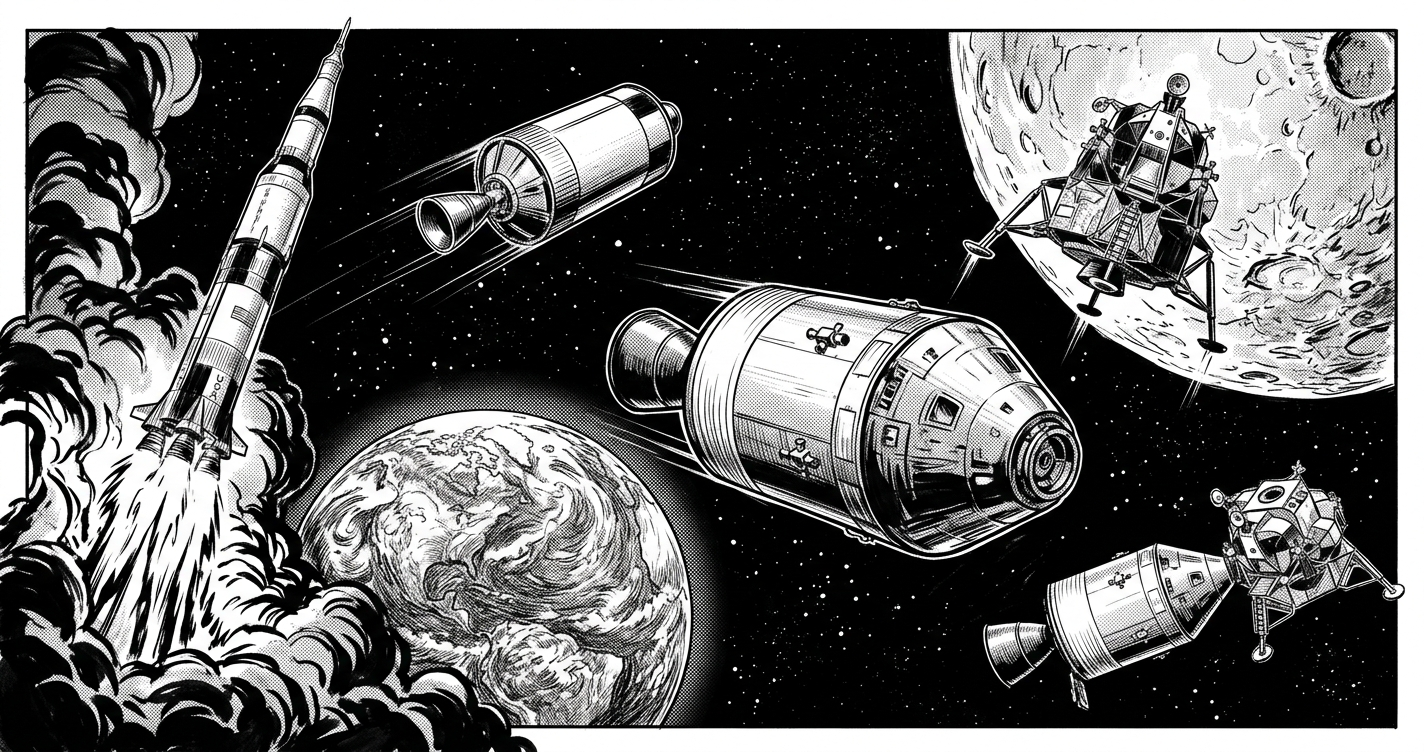
\includegraphics{apollo-comic-cover.png}%
}

\begin{document}
\begin{titlepage}
\centering
\vspace*{0.08in}
{\Huge\bfseries\sffamily APOLLO\par}
\vspace{0.1in}
{\LARGE\sffamily Hand-Calculation Outline\\[6pt]and Worked Answer Key\par}
\vspace{0.15in}
\resizebox{\linewidth}{!}{\ApolloCoverArt}\par
{\scriptsize Comic-book mission montage / AI-generated ink illustration / not to scale.\par}
\vspace{0.12in}
\begin{panel}{Mission Control copy --- keep answers covered}
Every mandatory calculation for the Apollo 11 beginner game and
Apollo 13 advanced game: inputs, equations, slide-rule procedures,
correct answers, decision gates, error consequences, and read-aloud
narration examples for Mission Control.
\end{panel}
\vspace{0.1in}
{\large 10 Apollo 11 checkpoints\\[6pt]10 Apollo 13 checkpoints\par}
\vfill
Companion player book: \texttt{apollo-game.pdf}\\[12pt]
Use guard digits to grade; expect about three significant figures
from a player. Do not demand calculator precision from a slide rule.
\\[20pt]
Historical schedules are cited. Invented telemetry and thresholds
are educational models, not NASA operational limits.
\end{titlepage}

\section*{Referee protocol and a worked error checkpoint}
Read the player book's full rules first. Apollo 11 starts with command
reserve 6; Apollo 13 starts with 4. Each card is graded on the
\emph{first committed sheet}; charge only its worst band once.
GREEN costs 0, AMBER 1, RED 2. Continue at zero, stop below zero.

\begin{panel}{Numerical bands}
Ordinary outputs:
\(\epsilon=100|q-q_{\rm ref}|/|q_{\rm ref}|\).
GREEN \(\leq1\%\), AMBER \(>1\%\) through \(5\%\), RED \(>5\%\).
Clock-format GET / intervals: GREEN within 1 s, AMBER through 60 s,
RED beyond. Computed decimal durations use relative bands.
Angles on 11-10, 13-08, 13-09: GREEN within \(0.05^\circ\),
AMBER through \(0.20^\circ\), RED beyond.
Wrong signs/quadrants, missing outputs, missing/incompatible units,
failed physical gates, or wrong discrete choices are RED.
\end{panel}

For physical gates, evaluate unrounded quantities. Do not mark a
correct rejected-profile negative remainder wrong merely because
it is negative. Only the \emph{selected} plan must meet the stated
constraint. The player must use the slide rule for the required
products, quotients, roots, and logarithms and record the work.

\textbf{Example: card 11-06.}
Crew commits fuel endurance 82.0 s, descent time 60.0 s, and chooses
the correct 20 s diversion. Reference endurance is 85.7142857 s;
\[
\epsilon=100\,|82.0-85.7142857|/85.7142857=4.33333\%.
\]
If all other outputs are GREEN, the checkpoint is \textbf{AMBER}.
Charge 1 reserve, narrate the less desirable landing site, and require
the corrected 85.7 s endurance / 25.7 s hover margin.

If the crew instead selects a 30 s diversion, the physical gate fails:
it needs \(0.700(60+30)=63.0\) kg but has only 60.0.
Grade \textbf{RED}, charge 2 once (not once per output), and narrate
the wave-off rehearsal. If reserve remains nonnegative, correct the
sheet and resume at the nominal landing baseline. If negative, stop
with the Apollo 11 safe lunar-orbit abort ending.

\textbf{State discipline.} Reserve and the Apollo 11 EVA narrative flag
are the only persistent error effects. Do not also consume invented
minutes, water, or fuel because of a warning.
All accepted pads must be corrected to GREEN quality before continuing.
Game failure is a simulation result, not a claim that the historical
crew failed.

\textbf{Read-aloud help.} The narration appendix starts on
page~\pageref{narration-start}. It includes launch and coast transitions,
briefings and GREEN / AMBER / RED examples for every card,
the cartridge-adapter scene, and all mission endings.
Read briefings before commitment; keep outcome scripts hidden until grading.

\Card{11-01}{Commit to the Moon}
{Planned TLI ignition 002:44:26; 320 s burn. [F1, Table 1-1]}
{Armstrong commands, Aldrin reads the burn pad, and Collins checks the
decimal place. The Saturn's third stage will send Columbia and Eagle
toward the Moon. Do not mistake feet per second for metres per second.}
{Convert the planned \(10{,}451.2\) ft/s velocity change to m/s.
Find its average acceleration over 5 min 20 s. Compute the cutoff GET.}
{Convert minutes by hand. On C/D multiply velocity by 0.3048, then divide
by elapsed seconds: \(\bar a=\Delta v/t\). Add the duration to GET on paper.
This is a whole-burn average, not constant actual thrust acceleration.}
{Write m/s, m/s\(^{2}\), and h:m:s on the pad. Missing or incompatible
units are RED. The modeled burn is commanded in the forward direction.}
{AMBER: guidance flags a targeting discrepancy; charge 1 reserve for a
corrective update. RED: the departure targeting test fails; charge 2 for
a simulator abort-and-replan. A depleted reserve here means a safe
Earth-orbit abort, not a lunar landing.}
{\(\Delta v=10{,}451.2(0.3048)=3185.52576\) m/s, so report
\(\boxed{3.19\times10^3\text{ m/s}}\).
\(t=5(60)+20=320\) s;
\(\bar a=3185.52576/320=\boxed{9.95\text{ m/s}^2}\).
Cutoff \(002{:}44{:}26+00{:}05{:}20=\boxed{002{:}49{:}46}\).
An estimate near \(10^4\) ft/s and \(3\times10^3\) m/s catches a factor-ten error.}

\Card{11-02}{Clear the spent stage}
{Planned evasive maneuver 004:39:44.9; 2.8 s. [F1, Table 1-1]}
{Collins separates the docked spacecraft from the spent stage.
The maneuver pad has two nonzero vector components, not two separate
burns. Mission Control wants a magnitude before authorizing ignition.}
{For \((\Delta v_x,\Delta v_y,\Delta v_z)=(5.1,0,19.0)\) ft/s,
find total velocity change in ft/s and m/s. A training model supplies
average acceleration \(2.14\) m/s\(^{2}\); find burn duration.}
{Square on A (or multiply C/D), add the squares with pencil, take the
square root on A/D:
\(\Delta v=\sqrt{\Delta v_x^2+\Delta v_y^2+\Delta v_z^2}\).
Convert on C/D and divide by \(\bar a\).}
{Use the vector magnitude, not \(5.1+19.0\).
Preserve the supplied component directions on the command pad.
The 2.14 m/s\(^{2}\) acceleration is invented training telemetry.}
{AMBER: separation is slower or faster than expected; charge 1 for a
tracking update. RED: the safe-separation prediction fails; charge 2
for an emergency avoidance rehearsal before continuing.}
{\(5.1^2+19^2=26.01+361=387.01\).
\(\Delta v=\sqrt{387.01}=19.67257\) ft/s
\(\rightarrow\boxed{19.7\text{ ft/s}}\).
\(\Delta v=19.67257(0.3048)=\boxed{6.00\text{ m/s}}\).
\(t=5.996199/2.14=\boxed{2.80\text{ s}}\), matching the
planned 2.8 s to slide-rule precision.
Use the table's vector / required-\(\Delta v\) data here, not the
different 15.6 ft/s value in its \(\Delta V_C\) column.}

\Card{11-03}{Capture lunar orbit}
{Planned LOI1 ignition 075:54:28.4; 358.9 s. [F1, Table 1-1]}
{Columbia passes behind the Moon. Houston cannot coach this burn in real
time. Collins reads a retrograde pad; the crew's arithmetic determines
whether the simulator accepts lunar capture.}
{Use components \((-2891.8,-433.1,+20.4)\) ft/s to find
\(\Delta v\) in ft/s and m/s. Find average acceleration for
5 min 58.9 s. Compute cutoff GET.}
{Use A/D for squares and roots, pencil for addition, C/D for unit
conversion and division. Use \(\bar a=\Delta v/t\).
Clock arithmetic is sexagesimal; keep the tenths of a second.}
{Keep all three component signs. A correct magnitude with reversed
retrograde direction is RED. This scalar exercise does not compute
an orbit or prove capture in the real world.}
{AMBER: tracking predicts an off-target lunar orbit; charge 1 for a
trim update. RED: the simulator rejects capture; charge 2 for a
contingency return rehearsal. Reserve exhaustion means abort the
landing and use the game's safe-return ending.}
{\(\Sigma \Delta v_i^2=8{,}550{,}499.01\) (ft/s)\(^{2}\).
Square root \(=2924.12363\) ft/s
\(\rightarrow\boxed{2.92\times10^3\text{ ft/s}}\).
Multiply by 0.3048 to get \(891.273\) m/s
\(\rightarrow\boxed{891\text{ m/s}}\).
\(t=358.9\) s and \(\bar a=891.273/358.9
=\boxed{2.48\text{ m/s}^2}\).
Cutoff \(075{:}54{:}28.4+00{:}05{:}58.9
=\boxed{076{:}00{:}27.3}\).
The table rounds required \(\Delta v\) to 2924.1 ft/s;
its separate \(\Delta V_C=2914.8\) ft/s is not substituted.}

\Card{11-04}{Work the lunar clock}
{Lunar-orbit operations between LOI2 and LM separation. [F1, p. 1-3]}
{Houston schedules a daylight observation and a radio call.
Collins must distinguish orbital night from loss of radio coverage:
they are different scheduling constraints.}
{An average orbit lasts 118.2 min, including 47 min of night.
Find daylight minutes, average angular rate in degrees/min,
and the percentage of an orbit with MSFN coverage if coverage is
72 min. Is a 65 min daylight task feasible in one daylight interval?}
{Subtract with pencil, then use C/D for \(360/118.2\) and
\(100(72/118.2)\). Compare the task with daylight duration.
Use the supplied full period, not the plan's rounded \(3^\circ/\)min.}
{The 65 min task must fit daylight. Do not treat 72 min of coverage as
72 min of daylight, or claim that their overlap is known.
The task duration is a training scenario.}
{AMBER: a mistimed observation loses useful coverage; charge 1 for
rescheduling. RED: the crew confuses the two windows and misses the
handover; charge 2 for a complete scheduling rebuild.}
{Daylight \(=118.2-47=\boxed{71.2\text{ min}}\).
Angular rate \(=360/118.2=\boxed{3.05^\circ/\text{min}}\).
Coverage \(=100(72/118.2)=\boxed{60.9\%}\).
\(\boxed{\text{GO}}\) for the daylight task:
\(71.2-65=\boxed{6.20\text{ min}}\) spare.
The plan gives approximately \(3^\circ/\)min; using the more precise
period explains the small difference. There is insufficient information
to require continuous radio contact throughout the task.}

\Card{11-05}{Lower Eagle's perilune}
{Planned DOI 101:38:48, 28.5 s; PDI 102:35:13. [F1, Table 1-2]}
{Aldrin checks descent-orbit insertion while Collins tracks Eagle.
Armstrong wants to know how much coast time remains after engine cutoff
before powered descent begins.}
{Use the table's required \(\Delta v=70.0\) ft/s.
Convert it to m/s; compute average acceleration over 28.5 s.
Find DOI cutoff GET and the coast interval from cutoff to PDI.}
{C/D handles conversion and \(\Delta v/t\).
Add the burn on paper, then subtract cutoff from PDI, borrowing
60 seconds or minutes when necessary.}
{Use required \(\Delta v\), not a reconstruction from the printed
components: this table's DOI components do not exactly reproduce 70.
The game does not resolve that source discrepancy.}
{AMBER: the coast briefing is late; charge 1 for an expedited pad
review. RED: a descent-readiness check is missed; charge 2 for a
full rehearsal. If reserve is exhausted, cancel PDI and rendezvous
with Columbia in the game's safe-return ending.}
{\(70(0.3048)=\boxed{21.3\text{ m/s}}\).
\(\bar a=21.336/28.5=\boxed{0.749\text{ m/s}^2}\).
Cutoff \(101{:}38{:}48+00{:}00{:}28.5
=\boxed{101{:}39{:}16.5}\).
PDI minus cutoff:
\(102{:}35{:}13-101{:}39{:}16.5
=\boxed{00{:}55{:}56.5}\).
The printed components \(67.46,-28.68,-12.51\) ft/s would give about
74.4 ft/s, so the specified 70.0 ft/s input is deliberate.}

\Card{11-06}{Land or wave off}
{Planned PDI 102:35:13 to touchdown 102:47:11. [F1, pp. 1-9, 3-69]}
{Armstrong sees a rough patch ahead. Aldrin calls altitude and fuel.
Choose the longest safe diversion before the checkpoint commits the
landing. This last-minute hover model is fictional, not Apollo telemetry.}
{First find touchdown GET and average whole-descent acceleration from
\(\Delta v=6766\) ft/s and 11 min 58 s.
At the terminal gate, altitude is 120 m and downward speed is held at
2.00 m/s. Fuel is 60.0 kg and consumption is 0.700 kg/s.
Find descent time, fuel endurance, and maximum extra hover time.
Choose the longest safe diversion from 10, 20, or 30 s; find fuel left.}
{Use C/D to convert velocity, divide for average acceleration,
divide altitude by speed, and divide fuel by flow.
Subtract endurance minus descent time. For a diversion \(d\),
\(m_{\rm left}=60-0.700(120/2+d)\).}
{Choose the longest listed diversion that leaves nonnegative fuel.
The terminal constant-speed model is separate from the whole-descent
average; do not use that average as net terminal acceleration.}
{AMBER: the landing pad needs a last-second correction; charge 1 and
land at a less desirable site. RED: fuel prediction rejects the
landing; charge 2 and rehearse an immediate wave-off. If reserve is
exhausted here, no landing occurs; end with a safe lunar-orbit abort.}
{Touchdown \(=\boxed{102{:}47{:}11}\).
\(t=718\) s; \(\Delta v=6766(0.3048)=2062.2768\) m/s;
\(\bar a=\boxed{2.87\text{ m/s}^2}\).
Terminal descent \(=120/2=\boxed{60.0\text{ s}}\).
Endurance \(=60/0.700=\boxed{85.7\text{ s}}\);
extra hover \(=85.7143-60=\boxed{25.7\text{ s}}\).
Choose \(\boxed{20\text{ s}}\).
Fuel left \(=60-0.700(80)=\boxed{4.00\text{ kg}}\).
A 30 s diversion would require 63 kg and is NO-GO.
Ten seconds is safe but not the requested longest safe choice.}

\Card{11-07}{A walk with a turnaround time}
{Planned EVA duration 2 h 40 min. [F1, p. 1-2]}
{Armstrong and Aldrin share the science work, but each carries an
independent oxygen budget. The flight director will not spend the
walk-back reserve on one more rock.}
{For each walker, oxygen starts at 1.80 kg; modeled use is
0.480 kg/h and protected reserve is 0.300 kg.
Find use and remaining oxygen over the 160 min EVA.
Find maximum allowed EVA duration and schedule margin.
Egress and return consume 28 min of the planned EVA; each science
station takes 12 min. How many complete stations fit?}
{C/D: convert minutes to hours, multiply by flow,
and divide usable oxygen by flow.
Pencil: subtract reserves and non-science time.
Round station count down, never up.}
{Both walkers must retain at least 0.300 kg.
The protected reserve is not available for science. These suit quantities
and task times are invented for play.}
{AMBER: Houston calls an early turnaround; charge 1 and record
``reduced science.'' RED: the oxygen or station plan violates a return
margin; charge 2 and record ``EVA curtailed.'' Correct the budget
before ascent preparations.}
{EVA \(=160/60=2.66667\) h.
Use \(=0.480(2.66667)=\boxed{1.28\text{ kg per walker}}\).
Remaining \(=1.80-1.28=\boxed{0.520\text{ kg}}\), so GO.
Allowed duration \(=(1.80-0.300)/0.480=3.125\) h
\(=\boxed{187.5\text{ min}}\) (3 h 7 min 30 s).
Margin \(=187.5-160=\boxed{27.5\text{ min}}\).
Stations \(=\lfloor(160-28)/12\rfloor=\boxed{11}\).
Do not divide one walker's tank by the combined two-person use rate.}

\Card{11-08}{Rise, meet, and dock}
{Planned ascent 124:23:26, 438 s; CSI 125:21:19.1. [F1, Table 1-2]}
{Eagle leaves the surface. Collins will bring Columbia to the rendezvous
only after Aldrin reads back ascent timing and a separate close-range
braking command.}
{For ascent \(\Delta v=6060\) ft/s, find m/s and average acceleration
over 7 min 18 s. Find insertion GET and time until CSI.
At the separate docking exercise, range is 40.0 m and closure speed
0.200 m/s. Find time to contact without braking and a burn duration
to cancel closure using \(0.0500\) m/s\(^{2}\).}
{Use C/D for conversion and division, pencil for GET.
For docking, \(t_{\rm contact}=r/v\) and \(t_{\rm brake}=\Delta v/a\).
The nominal burn is initiated immediately; stop the modeled closure
before contact and then let the referee narrate docking.}
{Command braking opposite to closure. Wrong direction is RED.
The close-range model is not the CSI maneuver and does not model
the actual rendezvous orbit.}
{AMBER: Collins delays docking while the crew corrects its pad; charge 1.
RED: the docking safety predictor flags a collision; charge 2 for an
emergency separation rehearsal. Exhaustion after landing means the
simulation ends with rendezvous unresolved, not an invented safe rescue.}
{\(\Delta v=6060(0.3048)=\boxed{1.85\times10^3\text{ m/s}}\).
\(\bar a=1847.088/438=\boxed{4.22\text{ m/s}^2}\).
Insertion \(124{:}23{:}26+00{:}07{:}18
=\boxed{124{:}30{:}44}\).
CSI coast \(125{:}21{:}19.1-124{:}30{:}44
=\boxed{00{:}50{:}35.1}\).
Time to contact \(=40/0.200=\boxed{200\text{ s}}\).
Braking \(=0.200/0.0500=\boxed{4.00\text{ s}}\), opposite closure.
During immediate uniform braking, travel is only
\(\tfrac12(0.200)(4)=0.400\) m, safely below the 40 m range.}

\Card{11-09}{Bring Columbia home}
{Planned TEI 135:24:33.8, 149.4 s; EI 195:03:27. [F1]}
{After docking and LM jettison, Collins checks the Earth-return pad.
Houston supplies signed components and the planned entry-interface
time, not a promise that every computed trajectory reaches Earth.}
{For components \((3213.3,705.0,-138.8)\) ft/s, find vector magnitude
in ft/s and m/s, and average acceleration over 2 min 29.4 s.
Find cutoff GET and coast time from cutoff to entry interface.}
{Use A/D to square and take a root; pencil to add;
C/D to convert and divide. Convert duration before adding GET.
Subtract the cutoff time, not ignition, from entry interface.}
{Retain the signed components on the burn command. An incorrect
direction is RED even with the right magnitude. Coast time is a
schedule calculation, not an orbital prediction.}
{AMBER: Earth-return targeting needs a trim; charge 1.
RED: the entry predictor rejects the pad; charge 2 for a return-burn
replan. Exhaustion means an unresolved return simulation.}
{\(\Sigma \Delta v_i^2=10{,}841{,}587.33\) (ft/s)\(^{2}\).
\(\Delta v=3292.65658\) ft/s
\(\rightarrow\boxed{3.29\times10^3\text{ ft/s}}\).
Multiply by 0.3048: \(\boxed{1.00\times10^3\text{ m/s}}\)
(guard value 1003.60172).
\(\bar a=1003.60172/149.4=\boxed{6.72\text{ m/s}^2}\).
Cutoff \(=\boxed{135{:}27{:}03.2}\).
Coast \(195{:}03{:}27-135{:}27{:}03.2
=\boxed{59{:}36{:}23.8}\).
The plan's rounded required magnitude is 3292.7 ft/s.}

\Card{11-10}{Entry corridor and recovery}
{Planned EI 195:03:27; detailed splashdown 13:55 later. [F1, p. 3-135]}
{The crew checks entry geometry before separating for the final descent.
Houston's training predictor supplies a downward vertical speed and a
horizontal speed. It is a diagnostic exercise, not an atmospheric model.}
{At the training gate, horizontal speed is 11.0 km/s and downward
vertical speed is 1.25 km/s. Find flight-path angle
\(\gamma=-\arctan(v_{\rm down}/v_{\rm horizontal})\), speed magnitude,
and kinetic energy per unit mass in MJ/kg.
Check the modeled corridor \(-6.8^\circ\leq\gamma\leq-6.2^\circ\)
and energy limit 63.0 MJ/kg. The detailed plan gives splashdown at
EI plus 13 min 55 s. Find splashdown GET and confirm the interval.}
{C/D gives the speed ratio; interpolate the tangent table on the
reference sheet or use T. Use A/D for speed.
\(e=v^2/2\): a squared speed in (km/s)\(^{2}\) gives MJ/kg directly.
Use pencil for clock subtraction.}
{Both corridor and energy checks must be GO. Positive \(\gamma\)
is an upward trajectory and is RED. These limits are game thresholds,
not authenticated Apollo flight rules.}
{AMBER: the predictor requests a corrected pad; charge 1.
RED: a shallow angle predicts skip-out, a steep angle predicts
excessive deceleration, or an energy error flags heating uncertainty;
charge 2. Do not enter until corrected. With reserve intact, narrate
parachutes and recovery; otherwise the return simulation is unresolved.}
{Ratio \(=1.25/11=0.113636\).
Table interpolation gives about \(6.48^\circ\);
\(\boxed{\gamma=-6.48^\circ}\).
\(v=\sqrt{11^2+1.25^2}=\boxed{11.1\text{ km/s}}\).
\(e=(121+1.5625)/2=\boxed{61.3\text{ MJ/kg}}\).
\(\boxed{\text{GO on both gates}}\).
Splashdown \(195{:}03{:}27+00{:}13{:}55
=\boxed{195{:}17{:}22}\).
Subtracting EI confirms \(\boxed{00{:}13{:}55}\).
The summary rounds this to 195:17; the game uses the more precise
detailed timeline rather than inventing zero seconds.}

\ifanswers\else
\clearpage
\section*{Apollo 13: change the mission, save the crew}
\begin{panel}{Advanced mission / fresh command reserve: 4}
Crew: Lovell, Haise, Swigert. Narrate successful launch, docking, and
outbound coast. At GET 055:54:53 the service-module oxygen-tank accident
occurs. The Moon is now a turning point, not a destination.
Your victory condition is recovery of all three crew after ten
corrected checkpoints, with command reserve still nonnegative.
\end{panel}

Unlike the Apollo 11 campaign, this mission requires independent
full-horizon consumable audits, a logarithmic rocket-equation
calculation, cartridge-count rounding, signed manual-navigation geometry,
and a linear entry-correction model.

\begin{tabularx}{\linewidth}{@{}lX@{}}
\toprule
Historical anchor & Event used in play\\
\midrule
055:54:53 & Oxygen-tank rupture; activate the LM lifeboat.\\
Near 061:30 & LM propulsion restores the desired free-return path.\\
079:27:39 & PC+2 begins after the lunar swingby.\\
Near 105:19 & Later manual correction; about a 15 s burn.\\
Final correction & A 22.4 s burn motivates the entry-predictor exercise.\\
141:30:02 & Aquarius jettison; Odyssey must already be ready.\\
142:54:41 & Historical splashdown and crew recovery.\\
\bottomrule
\end{tabularx}

\textbf{Planning epoch.} Consumable cards 13-03, 13-04, and 13-06 all
start their accounting at 058:00:00, regardless of when they are discussed
in the narrative. Plan the entire remaining horizon only once per pool.
Copy the time horizon to scrap paper and reuse it.

\textbf{Provenance.} The supplied PDF and text are both Apollo 11
resources. NASA's Apollo 13 catalog supplies these rescue event anchors.
All game inventories, simplified burn models, and failure thresholds
are invented and marked as training data.

\textbf{Before committing.} The commander checks direction, the LM
pilot checks the protected reserve, and the CM pilot checks time and
units. Any player may catch an error for free before ``commit.''
Start card 13-01 with a fresh ledger; do not carry Apollo 11 resources.
\fi

\Card{13-01}{The alarm: power the lifeboat}
{Historical tank rupture 055:54:53. [N1]; this activation model is invented.}
{Lovell takes command, Swigert powers down Odyssey, and Haise prepares
Aquarius. The explosion occurs regardless of your previous success.
Your objective changes from landing to bringing all three crew home.}
{In a separate emergency CM battery pool, usable energy is 2.40 kWh.
Load is 1.20 kW and LM activation takes 22 min.
Find initial endurance, activation energy, remaining energy,
and endurance remaining at that load. Find activation completion GET.
Is activation possible before this pool is exhausted?}
{Use C/D: \(t=E/P\), \(E=Pt\), minutes divided by 60.
Subtract energy on paper; add 22 min to the alarm time.
This emergency pool is not the protected entry battery on card 13-10.}
{Activate Aquarius immediately and transfer the crew.
Keeping Odyssey at this load indefinitely is NO-GO.
The explosion is a scripted historical event, never a penalty for bad math.}
{AMBER: transition checklist delays threaten battery margin; charge 1.
RED: the power-down budget is rejected; charge 2 for a contingency
transfer rehearsal. Reserve exhaustion means the rescue simulation fails.}
{Initial endurance \(=2.40/1.20=\boxed{2.00\text{ h}}\).
Activation \(=22/60=0.366667\) h;
energy \(=1.20(0.366667)=\boxed{0.440\text{ kWh}}\).
Remaining \(=2.40-0.440=\boxed{1.96\text{ kWh}}\).
Remaining endurance \(=1.96/1.20=\boxed{1.63\text{ h}}\)
(98 min).
Completion \(055{:}54{:}53+00{:}22{:}00
=\boxed{056{:}16{:}53}\).
\(\boxed{\text{GO}}\): 22 min is less than 120 min.}

\Card{13-02}{Restore a free return}
{Historical LM return maneuver near GET 061:30; magnitude 11.6 m/s. [N1]}
{The docked stack is not on the desired return path.
Haise reads a two-axis training pad while Lovell checks its direction.
This burn is distinct from the later PC+2 maneuver.}
{Training components are \((+11.0,+3.70)\) m/s.
Find total \(\Delta v\) and burn time using average acceleration
0.400 m/s\(^{2}\).
For a modeled constant thrust 12,000 N, \(I_{\rm sp}=305\) s,
and \(g_0=9.81\) m/s\(^{2}\), find mass flow and propellant used.}
{A/D handles vector magnitude. C/D:
\(t=\Delta v/\bar a\),
\(\dot m=F/(I_{\rm sp}g_0)\), \(m_{\rm used}=\dot m t\).
Keep intermediate readings on the sheet; do not repeatedly round them.
The fixed average acceleration is a supplied approximation.}
{Preserve both positive components. For this isolated maneuver,
usable propellant is 150 kg and at least 20 kg must remain.
Check the fuel gate; it is not the PC+2 tank inventory.}
{AMBER: return tracking predicts a correction; charge 1.
RED: a wrong-way or underbudgeted burn fails the free-return
predictor; charge 2 for a replanning rehearsal. No lunar landing is
available as an alternative ending.}
{\(\Delta v=\sqrt{11^2+3.7^2}
=\sqrt{134.69}=\boxed{11.6\text{ m/s}}\).
\(t=11.605602/0.400=\boxed{29.0\text{ s}}\).
\(\dot m=12{,}000/(305\cdot9.81)
=\boxed{4.01\text{ kg/s}}\).
\(m_{\rm used}=4.010629(29.014005)
=\boxed{116\text{ kg}}\) (guard value 116.364).
Remaining \(=150-116.364=\boxed{33.6\text{ kg}}\).
\(\boxed{\text{GO}}\), above the 20 kg reserve.
Mass and thrust values are training inputs, not the historical burn pad.}

\Card{13-03}{Three people, one oxygen budget}
{Game accounting epoch 058:00:00; historical splashdown 142:54:41. [N1]}
{Aquarius was designed for a different mission. Haise must choose a
conservation profile for the entire remaining flight. The same exact
time horizon will be used on the electrical and water cards.}
{Compute remaining flight time \(T\) in h:m:s and decimal hours.
LM usable oxygen is 12.0 kg with a protected 2.00 kg reserve.
Compare ``conserve'' use 0.0350 kg/(person h) against ``normal''
0.0500 kg/(person h), for three people.
Calculate total use and remaining oxygen for each; choose a safe profile.}
{Subtract GET on paper.
On C/D calculate \(T=84+54/60+41/3600\) and
\(m=3rT\). Subtract each use from 12.0 kg.
Keep \(T\) to at least four digits on paper for later cards.}
{Remaining oxygen must be at least 2.00 kg.
Do not confuse per-person use with total cabin use.
Carry the chosen profile to the mission ledger; all rates are
fictional planning averages.}
{AMBER: an incorrect budget prompts tighter rationing; charge 1.
RED: the selected profile cannot sustain the protected oxygen margin;
charge 2 for an emergency conservation replan.}
{\(142{:}54{:}41-058{:}00{:}00
=\boxed{84{:}54{:}41}\);
\(T=\boxed{84.9113889\text{ h}}\), normally read as 84.9 h.
Conserve: \(3(0.0350)T=\boxed{8.92\text{ kg}}\);
remaining \(\boxed{3.08\text{ kg}}\) (3.084304), GO.
Normal: \(3(0.0500)T=\boxed{12.7\text{ kg}}\);
remaining \(\boxed{-0.737\text{ kg}}\) (minus 0.736708), NO-GO.
Choose \(\boxed{\text{conserve}}\).
Its margin above the protected 2 kg is 1.084304 kg.}

\Card{13-04}{A dark, cold electrical plan}
{Same 058:00:00--142:54:41 horizon as 13-03.}
{Swigert asks which loads can remain off.
Haise proposes a low-power Aquarius profile; Lovell insists on
keeping entry energy protected rather than spending it on comfort.}
{Use \(T\) from 13-03. LM energy pool is 18.0 kWh; retain 2.50 kWh.
Non-idle operations cost 0.600 kWh in addition to idle use.
Compare idle loads 0.160 kW (low) and 0.240 kW (normal).
Find total use and remaining energy for each, and maximum permissible
idle power. Choose a profile.}
{C/D: \(E_{\rm use}=PT+0.600\).
Pencil: \(E_{\rm left}=18-E_{\rm use}\).
Then \(P_{\max}=(18-2.50-0.600)/T\).
Energy is kWh; power is kW. Do not multiply power by seconds here.}
{The low-power plan must retain at least 2.50 kWh.
The 0.600 kWh operations allowance already includes modeled LM burns;
do not charge them again. This pool is separate from CM entry energy.}
{AMBER: incorrect switching instructions force load shedding; charge 1.
RED: the chosen profile predicts depletion before recovery; charge 2
and rewrite the electrical plan. Cold and dim conditions are narrative
effects, not additional hidden resource deductions.}
{Low use \(=0.160(84.9113889)+0.600
=\boxed{14.2\text{ kWh}}\) (14.185822);
remaining \(\boxed{3.81\text{ kWh}}\).
Normal use \(=0.240T+0.600=\boxed{21.0\text{ kWh}}\);
remaining \(\boxed{-2.98\text{ kWh}}\).
\(P_{\max}=14.9/84.9113889
=\boxed{0.175\text{ kW}}\) (175.477 W).
Choose \(\boxed{\text{low}}\).
At 0.160 kW the reserve margin is 1.314178 kWh above 2.50.}

\Card{13-05}{PC+2: shorten the trip}
{Historical PC+2 ignition 079:27:39; burn 263.4 s, \(\Delta v=262\) m/s. [N1]}
{After passing the Moon, Aquarius must shorten the return.
This is the advanced slide-rule challenge: solve the rocket equation
backward, then compare the predicted duration with the historical anchor.}
{For a fictional mass model, \(m_0=30{,}000\) kg,
effective exhaust velocity \(v_e=3000\) m/s, target \(\Delta v=262\) m/s,
and average propellant flow 9.525 kg/s.
Find final mass, propellant used, and burn duration.
Find historical scheduled cutoff using 263.4 s, not your rounded prediction.}
{Use C/D and L:
\(x=\Delta v/(2.302585v_e)\),
\(m_f=m_0\,10^{-x}\),
\(m_{\rm used}=m_0-m_f\), \(t=m_{\rm used}/\dot m\).
On L, find the mantissa \(1-x\), read \(10^{1-x}\) on D,
then divide by 10 to obtain \(10^{-x}\).
Subtraction uses pencil; retain extra readable digits before subtracting.}
{The isolated burn's usable propellant is 2700 kg; retain 150 kg.
Mass must decrease, so \(m_f<m_0\). A wrong exponent sign is RED.
The historical time is an anchor; the masses and flow are invented.}
{AMBER: duration disagrees with the acceleration plan; charge 1 for a
throttle-pad correction. RED: the burn budget or exponent is wrong;
charge 2 for an emergency targeting rehearsal.}
{\(x=262/(2.302585\cdot3000)=0.03792838\).
\(10^{-x}=0.91637159\).
\(m_f=30{,}000(0.91637159)
=\boxed{27{,}491.15\text{ kg}}\) (slide-rule reading about 27,490).
Used \(=30{,}000-27{,}491.15
=\boxed{2508.85\text{ kg}}\), report \(2.51\times10^3\) kg.
\(t=2508.85237/9.525=\boxed{263\text{ s}}\)
(263.39657 s).
Remaining burn pool \(=2700-2508.85
=\boxed{191\text{ kg}}\), GO.
Historical cutoff \(079{:}27{:}39+00{:}04{:}23.4
=\boxed{079{:}32{:}02.4}\).
Allow the normal 1\% band on propellant despite subtractive sensitivity.}

\Card{13-06}{Cooling water versus drinking water}
{Same full return horizon \(T=84.9113889\) h; planning epoch 058:00:00.}
{Haise balances cooling against the crew's drinking allowance.
Choose a modeled cooling profile without borrowing the water
protected for entry and recovery.}
{Water starts at 100 kg; protect 12.0 kg.
Each of three crew uses 0.0600 kg/h for drinking.
Compare cooling 0.900 kg/h (normal) with 0.700 kg/h (reduced).
Find combined rates, total use, and water left for both profiles.
Find the maximum allowable cooling rate, then choose a safe profile.}
{C/D: \(r_{\rm total}=r_{\rm cool}+3r_{\rm drink}\),
\(m_{\rm use}=r_{\rm total}T\).
Subtract from 100 on paper.
\(r_{\rm cool,max}=(100-12)/T-3r_{\rm drink}\).}
{Keep at least 12.0 kg. Both proposed cooling settings are assumed
thermally permissible in this game; no thermal engineering calculation
is implied. The drinking allowance is not optional.}
{AMBER: a bad ration sheet prompts an uncomfortable reduced-cooling
replan; charge 1. RED: the selected profile consumes protected water;
charge 2 for emergency ration planning. Do not invent additional
water losses for narrative delays.}
{Drinking rate \(=3(0.0600)=0.180\) kg/h.
Normal total \(=\boxed{1.08\text{ kg/h}}\);
use \(=1.08T=\boxed{91.7\text{ kg}}\);
left \(\boxed{8.30\text{ kg}}\), NO-GO.
Reduced total \(=\boxed{0.880\text{ kg/h}}\);
use \(=0.880T=\boxed{74.7\text{ kg}}\);
left \(\boxed{25.3\text{ kg}}\), GO.
Maximum cooling \(=88/T-0.180
=\boxed{0.856\text{ kg/h}}\).
Choose \(\boxed{\text{reduced}}\).
Its margin above reserve is 13.277978 kg.}

\Card{13-07}{Make the square cartridge fit}
{Training checkpoint GET 090:00:00; CO\(_2\) planning to 134:00:00.}
{The astronauts need a cartridge adapter. The referee narrates its
construction from available materials; the mathematics determines
how many compatible cartridges and how soon they are needed.
This is not a real breathing-system construction guide.}
{Three people produce 0.900 kg of CO\(_2\) per person per day.
Existing compatible absorbent has 0.600 kg capacity remaining.
Each adapted spare removes 1.80 kg.
Find hourly production, the load for the next 44 h, and the minimum
integer number of spares needed in addition to existing capacity.
Find capacity margin, time until existing capacity runs out,
and the adapter deadline GET. Assembly takes 2.00 h: find time slack.}
{Use C/D for rate conversion and load.
Compute \(n=\lceil(m_{\rm load}-0.600)/1.80\rceil\): round UP.
Deadline \(t=0.600/r_{\rm hourly}\).
Add deadline to 090:00:00 and subtract assembly time on paper.}
{Finish the adapter before existing capacity expires and allocate enough
spares. Timing this card uses decimal endurance bands and clock bands;
cartridge count must be the exact minimum integer.}
{AMBER: a miscount requires inventory review; charge 1.
RED: the predicted scrubber gap would allow CO\(_2\) accumulation;
charge 2 for a rushed adapter rehearsal. The referee must not allow
the game to proceed with a knowingly inadequate scrubber plan.}
{Production \(=3(0.900)/24=\boxed{0.1125\text{ kg/h}}\).
Load \(=0.1125(44)=\boxed{4.95\text{ kg}}\).
\(n=\lceil(4.95-0.600)/1.80\rceil
=\lceil2.41667\rceil=\boxed{3\text{ spares}}\).
Capacity margin \(=0.600+3(1.80)-4.95
=\boxed{1.05\text{ kg}}\).
Existing endurance \(=0.600/0.1125
=\boxed{5.33333\text{ h}}\) (5 h 20 min).
Deadline \(=\boxed{095{:}20{:}00}\).
Assembly slack \(=5.33333-2=\boxed{3.33333\text{ h}}\)
(3 h 20 min). GO; finish by 092:00:00 if starting now.}

\Card{13-08}{Navigate without the usual computer}
{Historical correction near GET 105:19 used about a 15 s burn. [N1]}
{Lovell uses the visible Earth as an attitude reference.
Haise works the training pad by hand. There is no die roll for aim:
your signed vector and angle decide whether the predictor accepts it.}
{A fictional two-axis correction requires
\((\Delta v_x,\Delta v_y)=(-2.30,+0.400)\) m/s.
Find magnitude and burn time at average acceleration 0.155 m/s\(^{2}\).
Find angle above the negative \(x\) direction:
\(\theta=\arctan(0.400/2.30)\).
Write the commanded quadrant explicitly.}
{Use A/D for the vector root and C/D for division.
Use T, or interpolate the tangent table supplied on the reference sheet.
Signs define the quadrant; \(\theta\) is a small positive angle measured
from the negative \(x\) axis toward positive \(y\), not from positive \(x\).}
{Angle bands are GREEN within \(0.05^\circ\), AMBER through \(0.20^\circ\),
RED beyond. Wrong quadrant is always RED.
Magnitude and time still use ordinary relative-error bands.}
{AMBER: the predictor flags aim drift; charge 1 for an attitude reset.
RED: a wrong quadrant or angle predicts a missed entry corridor;
charge 2 for a complete manual-navigation rehearsal.}
{\(\Delta v=\sqrt{2.30^2+0.400^2}
=\sqrt{5.45}=\boxed{2.33\text{ m/s}}\).
\(t=2.3345235/0.155=\boxed{15.1\text{ s}}\).
Ratio \(=0.400/2.30=0.173913\).
T gives \(\boxed{9.87^\circ}\).
Table interpolation:
\(9.5+(0.173913-0.16734)/(0.17633-0.16734)(0.5)
=9.866^\circ\).
Command \(\boxed{\text{negative }x,\ \text{positive }y}\),
or about \(170.13^\circ\) counterclockwise from positive \(x\).
The historical maneuver's components are not being reconstructed.}

\Card{13-09}{Thread the entry corridor}
{Final historical correction lasted 22.4 s; game entry predictor is invented. [N1]}
{Swigert prepares Odyssey while Lovell checks the last correction.
The flight director supplies a locally linear response model.
It is deliberately simpler than a real Earth-entry trajectory.}
{Current modeled entry angle is \(-5.90^\circ\); target is
\(-6.50^\circ\). A positive corrective \(\Delta v\) changes angle by
\(-0.0400^\circ\) per m/s. Burn acceleration is 0.670 m/s\(^{2}\).
Find required \(\Delta v\), nominal burn duration, and predicted angle.
Find the minimum and maximum burn durations allowed by
\(-6.80^\circ\leq\gamma\leq-6.20^\circ\).}
{Use signed subtraction for \(\Delta\gamma\).
C/D: \(\Delta v=(\gamma_{\rm target}-\gamma_0)/k\) and
\(t=\Delta v/a\).
Repeat for both corridor edges.
Use \(\gamma(t)=\gamma_0+kat\) to check signs.}
{Command a positive correction with a negative angle response.
The nominal pad must target \(-6.50^\circ\), not merely any
duration in the corridor. Angle bands are \(0.05^\circ/0.20^\circ\).
Report the two duration bounds in ascending order.}
{AMBER: a small duration error produces a corridor warning; charge 1.
RED: a too-short burn predicts shallow skip-out; too long predicts
excessive entry loading. Charge 2 and correct before separation.}
{\(\Delta\gamma=-6.50-(-5.90)=-0.600^\circ\).
\(\Delta v=(-0.600)/(-0.0400)=\boxed{15.0\text{ m/s}}\).
\(t=15/0.670=\boxed{22.4\text{ s}}\);
\(\gamma=-5.90-0.0400(15)=\boxed{-6.50^\circ}\).
Shallow edge: \(\Delta v=7.50\) m/s,
\(t_{\min}=\boxed{11.2\text{ s}}\) (11.19403).
Steep edge: \(\Delta v=22.5\) m/s,
\(t_{\max}=\boxed{33.6\text{ s}}\) (33.58209).
Thus \(11.19403\leq t\leq33.58209\) s is the toy corridor.
The 22.4 s historical agreement is a chosen training calibration.}

\Card{13-10}{Wake Odyssey and come home}
{Historical LM jettison 141:30:02; splashdown 142:54:41. [N1]}
{Swigert powers Odyssey back up. Haise and Lovell check the final
energy plan before saying goodbye to Aquarius.
You must finish reactivation before jettisoning the lifeboat.}
{A separate, protected CM battery starts with 3.00 kWh.
Reactivation uses 0.800 kW for 45 min; entry 1.20 kW for 30 min;
recovery beacon 0.150 kW for 4.00 h.
Find each energy, total use, and energy remaining; retain 0.500 kWh.
Reactivation begins at 140:30:02: find completion GET and margin
until LM jettison. Find LM-jettison-to-splashdown interval.}
{Convert minutes to hours on C/D, then use \(E=Pt\).
Add energy with pencil; subtract from 3.00.
Add 45 min to reactivation GET and subtract the historical event times.
Beacon use extends after splashdown and is included in this pool.}
{Energy remaining must be at least 0.500 kWh and reactivation must
finish before 141:30:02. The CM battery was not charged for the
LM's earlier loads; do not merge those inventories.}
{AMBER: a sequencing error threatens the transfer; charge 1.
RED: premature jettison or insufficient entry energy fails the recovery
predictor; charge 2 and correct the sequence. If reserve remains
nonnegative and all gates are corrected, narrate parachutes and recovery
of all three crew. Otherwise end with rescue unproven.}
{Reactivation \(=0.800(45/60)=\boxed{0.600\text{ kWh}}\).
Entry \(=1.20(30/60)=\boxed{0.600\text{ kWh}}\).
Beacon \(=0.150(4)=\boxed{0.600\text{ kWh}}\).
Total \(=\boxed{1.80\text{ kWh}}\);
left \(=3.00-1.80=\boxed{1.20\text{ kWh}}\), GO.
Completion \(140{:}30{:}02+00{:}45{:}00
=\boxed{141{:}15{:}02}\).
Jettison margin \(=\boxed{00{:}15{:}00}\), GO.
Jettison to splashdown
\(142{:}54{:}41-141{:}30{:}02
=\boxed{01{:}24{:}39}\).
The power schedule is fictional; the separation and recovery anchors
come from the NASA catalog.}

\clearpage
\section*{Mission Control narration: how to use these scripts}
\label{narration-start}
\begin{panel}{Original game dialogue --- not historical quotations}
Everything in quotation marks in this appendix is invented read-aloud
dialogue or scene description. It is not a NASA transcript.
Use it verbatim or adapt it to your crew, without changing the inputs,
grading bands, resource rules, or historical event anchors.
\end{panel}

\textbf{Before a card.} Read its briefing below, announce the GET
printed on the calculation card, and read that card's telemetry and orders.
Where the card supplies no exact event time, name the phase instead;
do not invent a new deadline. Briefings intentionally omit answers.

\textbf{After commitment.} Grade first, subtract the appropriate
command-reserve charge once, and check the new reserve.
Read only the matching GREEN, AMBER, or RED example.
For an error, the examples below assume reserve is still nonnegative.
If reserve is negative, use the appropriate ending instead of inviting
another attempt. A correct sheet never receives a scripted error.

\textbf{Correction and continuation.} GREEN narration authorizes the
nominal game action. AMBER and RED narration hold that action pending a
corrected pad. After correction, use the common release line below,
then the card's GREEN scene where appropriate. For 11-06 AMBER, retain
the less desirable landing site; for 11-07 retain the recorded science
flag rather than announcing full science.

\begin{panel}{Reusable referee lines}
\textbf{Commitment:} ``Flight crew, give me your signed command,
units, and GO or NO-GO decision. Is that your committed pad?''

\textbf{AMBER bookkeeping:} ``That is an AMBER checkpoint.
One command-reserve point is charged. Your reserve is now
[read the ledger]. Revise the pad before we proceed.''

\textbf{RED bookkeeping:} ``That is a RED checkpoint.
Two command-reserve points are charged, once for this sheet.
Your reserve is now [read the ledger].''

\textbf{Release after correction:} ``The corrected pad is accepted.
There is no additional charge for this revision. Resume from this
card's nominal calculation baseline; keep the warning on the ledger.''

\textbf{Unmodeled passage of time:} ``We now advance to the next
card's supplied epoch. The intervening routine work is narrated;
no extra consumables are deducted.''
\end{panel}

\textbf{Predictions are not actual disasters.} Error scenes describe
the simulator's warning or contingency rehearsal. Do not narrate a
collision, exhausted tank, or atmospheric entry as having occurred
while players are still allowed to correct their commands.
No scene adds dice rolls, real-time pressure, hidden fuel charges, or
extra calculations. The cartridge scene is dramatic description,
not a breathing-apparatus construction procedure.

\clearpage
\section*{Apollo 11: launch and narrated transitions}
\textbf{Opening / before 11-01.}
``Armstrong, Aldrin, Collins: your mission is to land Eagle, complete
the planned surface work, and bring the crew home. The Saturn rises
through the cloud layer. Staging is nominal; Earth curves beneath you.
At planned GET 000:11:43, the spacecraft reaches its parking orbit.
For this game the launch is successful. Houston is preparing your
lunar-departure pad. Take out your pencils and slide rule.''

\textbf{After corrected 11-01 / before 11-02: docking and extraction.}
``The third-stage engine shuts down and the cabin settles into
weightlessness. Collins turns Columbia to face Eagle, eases toward
the docking target, and secures the connection. The lunar module is
extracted from the stage. That routine docking is narrated here,
not a new calculation checkpoint. Now the spent stage must be
left safely behind: prepare the avoidance pad.''

\textbf{After corrected 11-02 / before 11-03: translunar coast.}
``The spent stage recedes. Earth becomes a smaller blue disk while
the Moon grows ahead. The crew alternates navigation observations,
housekeeping, meals, and rest. Routine midcourse updates and thermal
control are handled in the narrated coast. Houston now sends the
lunar-capture pad. Check it before the Moon cuts off our radio link.''

\textbf{After corrected 11-03 / before 11-04: orbit operations.}
``Radio contact returns as Columbia comes around the Moon.
For the game's accepted capture branch, you are in lunar orbit.
The second orbit-insertion maneuver and routine LM inspection are
completed as narrated flight-plan operations. Collins has daylight
observations and communications to schedule; these are not the
same kind of window.''

\textbf{After corrected 11-04 / before 11-05: undock.}
``Armstrong and Aldrin complete Eagle's checkout.
Collins remains in Columbia, monitoring the separation.
The docking connection releases and the two vehicles drift apart.
Separation and activation are narrated operations here.
Eagle's next checkpoint is the burn that lowers its perilune.''

\textbf{After corrected 11-05 / before 11-06: descent readiness.}
``Eagle coasts toward the powered-descent point. Aldrin reviews the
corrected timing while Armstrong watches the surface move below.
Houston calls for the final descent-readiness check. No new coast
budget is charged. At the next card's terminal exercise, decide how
much diversion the supplied fuel model permits.''

\textbf{After corrected 11-06 / before 11-07: surface operations.}
``Eagle is settled on the surface in the accepted landing branch.
The crew completes the contact checks, secures the spacecraft,
and prepares for the planned walk. Collins continues his orbiting
watch. Before either walker leaves, Houston wants the oxygen
and science schedule checked.''

\textbf{After corrected 11-07 / before 11-08: prepare ascent.}
``The walkers return and secure the cabin. Record the science result
already earned; do not restore curtailed work.
Equipment stowage, rest, and ascent preparations are narrated.
Collins is ready in Columbia. Eagle's crew must now check ascent
timing and the separate close-range braking exercise.''

\textbf{After corrected 11-08 / before 11-09: jettison.}
``The corrected approach brings the docking targets together.
Contact, capture, and a secure connection are confirmed.
Armstrong and Aldrin transfer back to Columbia.
The LM-jettison sequence and separation maneuver are narrated
without another calculation. All three crew now prepare
the trans-Earth injection pad.''

\clearpage
\section*{Apollo 13: launch, crisis, and narrated transitions}
\textbf{Opening / before 13-01.}
``Lovell, Haise, Swigert: the original mission is a lunar landing.
Launch, Earth-orbit checkout, lunar departure, and docking are
successful for this game. Odyssey and Aquarius head outward together.
Routine coast operations pass without a calculation checkpoint.
Now announce GET 055:54:53: a sharp disturbance runs through the
spacecraft, and warning indications appear on the panels.
Something has failed in the service module. The landing mission is
over; your new mission is to bring three people home.''

\textbf{After corrected 13-01 / before 13-02: transfer.}
``Odyssey's nonessential loads go dark.
Haise brings Aquarius into its lifeboat role while Swigert preserves
the command module for later. The crew moves through the connecting
tunnel with checklists and essential equipment.
Houston now needs a return maneuver that the LM engine can perform
with the two spacecraft still docked.''

\textbf{After corrected 13-02 / before 13-03--04: planning audit.}
``The accepted correction puts the simulator on its return branch.
Houston and the crew spread out the consumable sheets.
The oxygen and power audits both start their accounting at
058:00:00, even though this discussion follows the maneuver scene.
They cover the whole remaining trip; they are not fresh snapshots
or deductions from an already-used inventory.''

\textbf{After corrected 13-04 / before 13-05: lunar swingby.}
``Aquarius is quiet and dim under the accepted conservation plan.
The Moon fills the windows and then passes behind the docked stack.
For a time there is no radio contact. When Houston's voice returns,
the crew prepares PC+2: the major burn intended to shorten the trip
and improve the return target. Read the mass model carefully.''

\textbf{After corrected 13-05 / before 13-06: return coast.}
``The burn ends and Earth becomes the destination ahead.
The crew settles back into the low-power return coast.
Houston now reviews cooling and drinking water.
This is another audit of the same full horizon starting at 058:00:00,
not an extra charge for the time just narrated.''

\textbf{At 13-07: cartridge-adapter assembly.}
Read the briefing and telemetry, then grade the committed plan.
Only after the plan is accepted or corrected, read:
``Haise lays out the spare cartridges and the materials available
in the cabin. Swigert reads the simulated ground instructions while
Lovell holds the parts steady in weightlessness.
The crew assembles the adapter during the card's stated assembly
interval. For this game, the adapter connects the allocated
cartridges to the airflow path and the capacity plan is accepted.
No extra crafting roll or chemical calculation is required.''

\textbf{After corrected 13-07 / before 13-08--09: manual navigation.}
``The adapted scrubber arrangement is working in the accepted game
branch. With the ordinary guidance setup unavailable for this
exercise, Lovell uses the visible Earth as an attitude reference.
Haise reads the signed correction pad, and Swigert checks the units.
The later entry predictor will ask a different question:
how long must the final correction last?''

\textbf{After corrected 13-09 / before 13-10: ready Odyssey.}
``The corrected entry pad is accepted.
The damaged service module is separated in the narrated sequence.
Swigert prepares to wake Odyssey while Aquarius is still available.
Do not jettison the lifeboat until the final card's energy and
reactivation timing gates have been accepted.''

\newcommand{\NarrationCard}[6]{%
  \subsection*{#1 --- #2}
  \textbf{Briefing (before calculation):} ``#3''\par
  \textbf{GREEN (accepted command):} ``#4''\par
  \textbf{AMBER (charge 1, then correct):} ``#5''\par
  \textbf{RED (charge 2; if reserve permits, then correct):} ``#6''\par}

\clearpage
\section*{Apollo 11 checkpoint scripts / 11-01--02}
\NarrationCard{11-01}{Commit to the Moon}
{Houston to Columbia: we are at the lunar-departure gate.
Aldrin, read the velocity units. Collins, check the duration and
decimal place. Armstrong, hold the command until the crew commits.}
{The departure pad is accepted. The third stage lights, acceleration
builds, and the burn ends on the checked clock.
Columbia and Eagle begin the game's outbound lunar coast.}
{Guidance review has flagged a targeting discrepancy.
We need a corrective update before accepting the departure pad.
Check your unit conversion, average acceleration, and cutoff time.}
{The simulator rejects this departure solution.
Run the abort-and-replan rehearsal; do not execute this pad.
If command reserve permits, rebuild the calculation and read it back.}

\NarrationCard{11-02}{Clear the spent stage}
{Columbia, the docked spacecraft is clear of the extraction sequence,
but the stage is still nearby. Read the vector as one maneuver,
then tell Houston its magnitude and commanded duration.}
{The safe-separation predictor accepts your pad.
The short maneuver sends the spent stage steadily away.
The crew can turn its attention to the coast ahead.}
{The predicted separation rate differs from the accepted model.
Houston requests a tracking update and corrected magnitude.
Keep the component directions on the revised pad.}
{The safe-separation check fails. Rehearse emergency avoidance in
the simulator; no collision has occurred in the game.
Rebuild the vector and duration before proceeding.}

\clearpage
\section*{Apollo 11 checkpoint scripts / 11-03--04}
\NarrationCard{11-03}{Capture lunar orbit}
{The Moon is about to block Houston's signal.
Collins, verify the retrograde signs; Aldrin, check the magnitude
and cutoff clock. Your committed pad must stand on its own.}
{The engine shuts down at the accepted cutoff.
As the spacecraft emerges from behind the Moon, radio contact
returns. The simulator accepts lunar capture.}
{Tracking predicts an off-target lunar orbit.
Houston requests a trim update. Correct the signed pad and timing
before we accept the nominal capture branch.}
{The simulator rejects lunar capture with this pad.
Prepare the contingency-return rehearsal.
If reserve remains, correct the burn solution before resuming.}

\NarrationCard{11-04}{Work the lunar clock}
{Collins, sunlight and radio coverage are separate constraints.
Houston needs the observation schedule checked against daylight,
not against a coverage duration that happens to look similar.}
{The daylight task fits, and the schedule is accepted.
Record the coverage fraction separately; we have not assumed
that the entire observation has continuous radio contact.}
{The observation timing would lose useful coverage.
Houston requests a revised schedule. Recheck the orbit period,
daylight interval, and coverage percentage independently.}
{The handover schedule is rejected.
Rebuild the scheduling sheet; do not substitute a radio window
for a daylight window. The missed handover is a simulator contingency.}

\clearpage
\section*{Apollo 11 checkpoint scripts / 11-05--06}
\NarrationCard{11-05}{Lower Eagle's perilune}
{Eagle, Houston wants descent-orbit insertion checked before ignition.
Use the required velocity change specified on this card, then tell
us when cutoff occurs and how much coast remains before PDI.}
{The DOI pad is accepted.
The burn ends on the corrected clock, and Eagle enters the
game's descent coast with its readiness interval accounted for.}
{The coast briefing would be late on this sheet.
Expedite the pad review in the narrative, then correct the cutoff
and coast interval. No extra fuel or elapsed-time charge is added.}
{The descent-readiness check fails.
Rehearse the full readiness sequence before attempting PDI.
If reserve remains, correct the sheet and resume the nominal coast.}

\NarrationCard{11-06}{Land or wave off}
{Armstrong sees a rough patch ahead; Aldrin watches altitude and fuel.
Check the supplied terminal model and choose the longest listed
diversion that still permits descent without exhausting the fuel.}
{The chosen diversion passes the fuel gate.
Eagle moves toward the selected patch, descends, and settles.
The crew reports contact and secures the spacecraft.}
{The landing pad needs a last-second correction.
Correct the calculation before touchdown is accepted.
In the accepted continuation, Eagle lands at a less desirable site;
the warning remains on the ledger.}
{The fuel predictor rejects the landing command.
Rehearse an immediate wave-off; the game has not committed touchdown.
If reserve remains, correct the diversion choice and landing pad.}

\clearpage
\section*{Apollo 11 checkpoint scripts / 11-07--08}
\NarrationCard{11-07}{A walk with a turnaround time}
{The hatch is ready, but Houston wants the return margin protected.
Budget each walker's oxygen separately, then check how many
complete science stations fit the planned EVA.}
{The EVA plan is accepted. The walkers work through the planned
science schedule and return with the protected margin intact.
Record full planned science if no warning occurred on this card.}
{Houston calls for an early turnaround.
Record reduced science, then correct the oxygen and station sheet.
The crew returns safely in the accepted continuation, but the
lost science is not restored by the correction.}
{The plan violates the modeled return margin.
Record EVA curtailed and rehearse the immediate return.
Correct the sheet before ascent preparations; do not claim that
the original full science schedule was completed.}

\NarrationCard{11-08}{Rise, meet, and dock}
{Eagle's ascent pad is on the desk.
Check insertion timing first. Then work the separate close-range
exercise: how long before contact, and which way must you brake?}
{Ascent timing and braking are accepted.
Eagle reaches the game's rendezvous branch; the closing motion
is canceled. The docking targets align, contact is made,
and the connection is secured.}
{Collins holds the docking approach while the crew corrects its pad.
Check the insertion clock and braking duration.
The narrative delay adds no hidden propellant charge.}
{The docking predictor flags a possible collision.
Rehearse emergency separation in the simulator; no impact is
declared. Correct the braking direction and pad before docking.}

\clearpage
\section*{Apollo 11 checkpoint scripts / 11-09--10}
\NarrationCard{11-09}{Bring Columbia home}
{All three crew are back aboard Columbia.
Houston has supplied the Earth-return components and entry clock.
Read the signs, compute the magnitude, and measure coast from cutoff.}
{The return pad is accepted.
The engine fires and shuts down on the checked clock.
The simulator advances Columbia onto its nominal Earth-return branch.}
{Return targeting calls for a trim update.
Review the vector magnitude, acceleration, and cutoff-to-entry
interval before we accept the corrected departure.}
{The entry predictor rejects the return pad.
Rehearse a return-burn replan and correct the signed command.
Do not announce a successful Earth return until the later gates pass.}

\NarrationCard{11-10}{Entry corridor and recovery}
{Earth fills the window. Houston's training predictor supplies
horizontal and downward speeds. Check both the angle corridor
and energy gate before the game commits entry.}
{Both entry checks pass.
In the accepted branch, the capsule descends, the parachutes open,
and Columbia reaches the water on the planned game schedule.
Read the successful Apollo 11 ending once all corrected gates pass.}
{The predictor requests a corrected entry pad.
Hold the entry narration while you revise the angle, energy,
or clock result. Recovery is narrated only after acceptance.}
{This pad is not accepted for entry.
A shallow-angle error warns of skip-out; a steep-angle error warns
of excessive deceleration; an energy error raises heating uncertainty.
Use only the warning that fits this sheet, then correct if reserve permits.}

\clearpage
\section*{Apollo 13 checkpoint scripts / 13-01--02}
\NarrationCard{13-01}{The alarm: power the lifeboat}
{Warning lights are appearing after the service-module accident.
Swigert, check the emergency battery endurance.
Haise, prepare Aquarius. Lovell, authorize the transfer only after
the activation and power-down plan has been checked.}
{The transfer plan is accepted.
Odyssey's nonessential loads are shut down, Aquarius comes online,
and the crew moves into the lifeboat on the checked schedule.}
{The transition checklist threatens the battery margin.
Revise the activation and remaining-energy figures before the
transfer plan is accepted. The accident itself is not your penalty.}
{The power-down budget is rejected.
Rehearse the contingency transfer and correct the pad.
Keeping Odyssey at the emergency load indefinitely is not a rescue plan.}

\NarrationCard{13-02}{Restore a free return}
{Houston needs a return maneuver with the spacecraft still docked.
Haise, work the two-axis pad; Lovell, check direction.
Swigert, confirm that the modeled fuel reserve survives the burn.}
{The free-return pad passes the model's checks.
Aquarius performs the accepted correction.
Houston can now plan the remaining rescue around this return branch.}
{Return tracking predicts a correction.
Review the vector magnitude, burn duration, and fuel estimate
before accepting the nominal maneuver.}
{The free-return predictor rejects this command.
Rehearse the targeting replan, preserving the supplied directions.
There is no lunar-landing alternative in this rescue mission.}

\clearpage
\section*{Apollo 13 checkpoint scripts / 13-03--04}
\NarrationCard{13-03}{Three people, one oxygen budget}
{Aquarius must support three people for the remaining trip.
These are full-horizon planning figures from the stated epoch.
Compare both profiles and choose one that protects the oxygen reserve.}
{The conservation profile and budget are accepted.
The ledger shows oxygen protected for the return.
Keep this corrected plan; do not subtract the full horizon a second time.}
{Houston asks for a tighter ration-sheet review.
Correct the time horizon and total crew use before proceeding.
The warning does not create a new oxygen loss.}
{The selected profile cannot protect the modeled oxygen margin.
Replan conservation immediately in the simulator.
A profile that depletes the pool is not accepted just because
its arithmetic is written neatly.}

\NarrationCard{13-04}{A dark, cold electrical plan}
{The cabin can be quiet and dim, but the accepted plan must keep
energy protected. Separate idle power from the operations allowance
and check the whole return horizon.}
{The low-power plan is accepted.
Unneeded loads stay off while the required systems remain in
the game plan. The crew settles into the dim return coast.}
{The switching sheet needs load shedding.
Correct the power and energy budget; keep the reserve protected.
The colder, darker cabin is narration, not a second numerical penalty.}
{The chosen profile predicts depletion before recovery.
Rewrite the electrical plan before continuing.
Do not borrow the separate command-module entry battery to hide the error.}

\clearpage
\section*{Apollo 13 checkpoint scripts / 13-05--06}
\NarrationCard{13-05}{PC+2: shorten the trip}
{The lunar swingby is behind you.
Houston needs PC+2 checked with the supplied mass model.
Use the logarithmic scale carefully: propellant use must reduce mass.}
{The burn budget is accepted.
Aquarius fires through the planned PC+2 interval and shuts down
at the historical schedule anchor. The game's return branch
now continues toward Earth.}
{The duration differs from the accepted model.
Houston requests a throttle-pad correction.
Recheck the logarithm, subtraction, and division before the burn is accepted.}
{The burn budget or exponent fails the targeting check.
Rehearse emergency targeting and rebuild the mass calculation.
Do not command a model in which the spacecraft gains mass by burning fuel.}

\NarrationCard{13-06}{Cooling water versus drinking water}
{Haise has cooling requirements on one sheet and drinking allowance
on another. Combine the rates for the entire return horizon
without spending the water protected for entry and recovery.}
{The reduced-cooling profile passes the game water gate.
Record the accepted total and remaining water.
The crew continues with the card's drinking allowance preserved.}
{The ration sheet requires an uncomfortable reduced-cooling replan.
Correct the rates and remaining water before proceeding.
The narrative does not subtract additional water.}
{The selected profile consumes protected water.
Rehearse emergency ration planning, then correct the cooling choice.
The three-person drinking allowance cannot be erased to make the sheet pass.}

\clearpage
\section*{Apollo 13 checkpoint scripts / 13-07--08}
\NarrationCard{13-07}{Make the square cartridge fit}
{Houston has an adapter concept for the available cartridges.
Before we narrate assembly, count the required spares and determine
when the existing capacity runs out. Round capacity needs upward.}
{The cartridge allocation and assembly timing pass.
Read the adapter-assembly transition scene.
The accepted capacity plan covers this card's stated interval.}
{The inventory sheet needs review.
Recheck the production rate, allocation, or deadline before assembly
is accepted. A wrong minimum integer count is RED, not merely AMBER.}
{The plan fails the allocation or timing gate.
A scrubber gap would allow carbon-dioxide accumulation in the model.
Rehearse the rushed adapter contingency, then correct the plan
before narrating successful assembly.}

\NarrationCard{13-08}{Navigate without the usual computer}
{Lovell has Earth in view as the exercise's attitude reference.
Haise reads the correction pad.
The angle is measured from negative x toward positive y;
check the quadrant before committing.}
{The signed manual-navigation pad is accepted.
Lovell holds the reference while Haise calls the burn interval.
The simulator accepts the correction toward the entry target.}
{The aim predictor flags drift.
Reset the modeled attitude and correct the angle or burn duration.
Do not change the reference axis to make the result look smaller.}
{The predictor rejects the direction or angle.
A wrong quadrant could miss the entry corridor.
Rehearse manual navigation from the reference again and correct
the signed pad before continuing.}

\clearpage
\section*{Apollo 13 checkpoint scripts / 13-09--10}
\NarrationCard{13-09}{Thread the entry corridor}
{Houston's local predictor says the current approach needs adjustment.
Find the nominal correction and the two corridor bounds.
The supplied angle response is negative for a positive correction.}
{The nominal pad targets the accepted entry angle.
The simulator accepts the final correction.
The crew can now prepare Odyssey's reactivation sequence.}
{The duration produces a corridor warning.
Correct the nominal pad and both bounds before proceeding.
Being somewhere inside the toy corridor does not replace the requested target.}
{The correction pad is rejected.
Too little modeled correction warns of a shallow approach;
too much warns of excessive entry loading.
Select the applicable warning and rework the signed duration solution.}

\NarrationCard{13-10}{Wake Odyssey and come home}
{Swigert is ready to power Odyssey back up.
Haise and Lovell check the protected battery and completion clock.
Aquarius must remain attached until the accepted reactivation is complete.}
{The energy and timing gates pass.
Odyssey is ready before Aquarius is released.
In the accepted branch, the capsule enters, parachutes deploy,
and the crew reaches the water. Read the successful rescue ending.}
{The transfer sequence needs correction.
Hold the jettison narration while you revise the energy or timing sheet.
No successful recovery is announced until the gates are accepted.}
{The recovery predictor rejects the sequence or battery plan.
Premature jettison or insufficient entry energy would compromise
the modeled return. Correct the plan if reserve remains;
otherwise use the failed-rescue simulation ending.}

\clearpage
\section*{Mission endings: read only the earned branch}
\textbf{Apollo 11 / all ten corrected gates; \(R\geq0\).}
``Columbia is on the water. Recovery crews reach the capsule and
the flight crew is brought aboard. Eagle landed, and the crew came
home. Your mission result is crew recovered; landing achieved.''
Then read exactly one science result:
\begin{itemize}
\item No 11-07 warning: ``The record shows full planned science.''
\item 11-07 AMBER: ``An early turnaround reduced the science return;
the record keeps that warning despite the corrected budget.''
\item 11-07 RED: ``The EVA was curtailed to protect the return margin;
the record does not claim the full science schedule.''
\end{itemize}

\textbf{Apollo 11 / \(R<0\) on 11-01 or 11-02.}
``Command reserve is exhausted at the departure or avoidance checkpoint.
Stop the scored run. The training scenario takes its safe Earth-orbit
abort ending; the lunar landing is canceled.
This is a narrated game branch, not a calculated return trajectory.''

\textbf{Apollo 11 / \(R<0\) on 11-03 through 11-06.}
``Command reserve is exhausted before an accepted landing.
Houston cancels the descent mission. The training scenario takes
its safe-return contingency ending; Eagle does not land.
No later calculation can convert this scored abort into a completed mission.''
For 11-05 or 11-06, optionally add:
``The scenario narrates Eagle returning to Columbia rather than
continuing the landing attempt.''

\textbf{Apollo 11 / \(R<0\) on 11-07 through 11-10.}
``The simulation stops here with command reserve exhausted.
We have not established a completed rendezvous or return, as applicable
to this checkpoint. Record simulation terminated; return or rendezvous
unresolved. Do not narrate an automatic rescue of a landed crew.''

\textbf{Apollo 13 / all ten corrected gates; \(R\geq0\).}
``Odyssey is on the Pacific. Recovery personnel reach the capsule,
and Lovell, Haise, and Swigert are brought to safety.
There was no lunar landing, but the rescue mission achieved its goal:
all three crew recovered. Record the remaining command reserve
as your team's command-quality result, not a survival probability.''

\textbf{Apollo 13 / \(R<0\) at any checkpoint.}
``Command reserve is exhausted. Stop the rescue simulation at this
checkpoint; the game has not established crew survival.
Record rescue simulation failed; crew survival not established.
This result does not change history: the actual Apollo 13 crew returned safely.''

\clearpage
\section*{Sources, provenance, and modeling boundaries}
\textbf{[F1] Supplied Apollo 11 flight-plan resources.}
NASA Manned Spacecraft Center, \emph{Apollo 11, AS-506/CSM-107/LM-5,
Final Flight Plan}, July 1, 1969.
Local files: \texttt{Apollo11\_Flight\_Plan.pdf} (353 PDF pages)
and \texttt{flight\_plan.txt}.
The text rendition is not an Apollo 13 flight plan.
Printed section page numbers below are preferable to text-file line
numbers, which change with extraction format.

\begin{tabularx}{\linewidth}{@{}lX@{}}
\toprule
Source location & What is used\\
\midrule
pp. 1-1--1-3 & Phase order; orbit insertion; EVA duration;
118.2 min lunar orbit, 47 min night, 72 min MSFN coverage;
summary entry / splashdown schedule.\\
Figure 1-3, p. 1-7 & Powered-descent structure; high/low gates motivate
the fictional terminal landing decision.\\
Table 1-1, p. 1-8 & CSM ignition times, burn durations, and supplied
vector components for TLI, avoidance, LOI, and TEI. PDF page 30.\\
Table 1-2, p. 1-9 & DOI, PDI, ascent, and CSI timing; required
velocity changes. PDF page 31.\\
Detailed timeline, p. 3-69 & PDI 102:35:13, burn 11:58,
touchdown 102:47:11.\\
Detailed timeline, p. 3-135 & Entry interface 195:03:27,
more precise than the summary's 195:03; splashdown EI plus 13:55,
giving 195:17:22.\\
\bottomrule
\end{tabularx}

\textbf{[N1] Supplemental Apollo 13 history.}
NASA Space Science Data Coordinated Archive,
\emph{Apollo 13 Command and Service Module}, catalog ID 1970-029A,
``Mission Profile,'' accessed October 2, 2026.
\url{https://nssdc.gsfc.nasa.gov/nmc/spacecraft/display.action?id=1970-029A}

This source documents the accident at GET 55:54:53, transfer to the LM,
an 11.6 m/s return maneuver, the 263.4 s / 262 m/s PC+2 burn,
an approximately 15 s later correction, a 22.4 s final correction,
LM jettison, and splashdown at GET 142:54:41.
Times given in UTC are converted from launch at April 11, 1970,
19:13:00 UTC: PC+2 April 15 at 02:40:39 becomes 079:27:39;
LM jettison April 17 at 16:43:02 becomes 141:30:02.
The April 16 correction at 04:32 UTC is near 105:19 GET;
the game does not present it as an exact ignition timestamp.

\textbf{What is invented.} Emergency and entry battery pools, resource
inventories and rates, allowable reserves, simplified thrust / mass
models, docking range and speed, terminal landing fuel and altitude,
science-station durations, cartridge capacities, manual-navigation
components, entry geometry and linear response, checkpoint bands,
command reserve, and every error consequence are game design.
No supplied Apollo 13 flight plan was available.
Historical Apollo 13 event anchors supplement the Apollo 11 plan's
flight-planning structure; its rescue path is not an Apollo 11 timeline
with names changed.

\textbf{Limits.} No numerical model here predicts a true orbit,
real atmospheric heating, scrubber chemistry, or mission survival.
Fixed rates and average acceleration are intentional educational
approximations. All real missions required substantial ground and
onboard computation; this game does not claim they were flown using
only a slide rule.

\end{document}
